\documentclass{article}
\usepackage{graphicx}
\usepackage{fancyhdr}
\usepackage{hyperref}
\usepackage{float}
\hypersetup{
  colorlinks   = true,
  urlcolor     = blue,   
  linkcolor    = blue,     
}

%page setup- title and author
\title{Project Phase 1}
\author{Team 025}
\pagestyle{fancy}

%header and footer
\fancyhf{}
\fancyhfoffset[L]{1cm}
\fancyhfoffset[R]{1cm}
\lhead{Phase 1 Report}
\chead{CS 6400 - Spring 2025}
\rhead{Team 025}
\lfoot{\hyperlink{toc}{Table of Contents}}
\rfoot{\thepage}

%table of contents
\begin{document}
\maketitle
\tableofcontents
\newpage

\section{Data Types}

\noindent\textbf{Dog}
\begin{table}[H]
    \begin{tabular}{|l|l|l|}
    \hline
    \textbf{Attribute}         & \textbf{Data Type}                  & \textbf{Nullable} \\ \hline
    BirthDate                  & Date                                & Not Null          \\ \hline
    DogID                      & Integer                             & Not Null          \\ \hline
    Description                & String                              & Null              \\ \hline
    Altered                    & Boolean                             & Not Null          \\ \hline
    Sex                        & String                              & Not Null          \\ \hline
    Name                       & String                              & Not Null          \\ \hline
    SurrenderDate              & Date                                & Not Null          \\ \hline
    SurrenderPhone             & String                              & Null              \\ \hline
    ByAnimalControl            & Boolean                             & Not Null          \\ \hline
    \end{tabular}
\end{table}

\noindent \textbf{Breed}
\begin{table}[H]
    \begin{tabular}{|l|l|l|}
    \hline
    \textbf{Attribute}        & \textbf{Data Type} & \textbf{Nullable} \\ \hline
    Name                      & String             & Not Null          \\ \hline
    \end{tabular}
\end{table}

\noindent \textbf{Microchip}
\begin{table}[H]
    \begin{tabular}{|l|l|l|}
    \hline
    \textbf{Attribute}        & \textbf{Data Type} & \textbf{Nullable} \\ \hline
    MicrochipID               & String            & Not Null          \\ \hline
    \end{tabular}
\end{table}

\noindent \textbf{Manufacturer}
\begin{table}[H]
    \begin{tabular}{|l|l|l|}
    \hline
    \textbf{Attribute}        & \textbf{Data Type} & \textbf{Nullable} \\ \hline
    Name                      & String             & Not Null          \\ \hline
    \end{tabular}
\end{table}

\noindent \textbf{Expense}
\begin{table}[H]
    \begin{tabular}{|l|l|l|}
    \hline
    \textbf{Attribute}   & \textbf{Data Type} & \textbf{Nullable} \\ \hline
    Amount               & Float              & Not Null          \\ \hline
    Vendor               & String             & Not Null          \\ \hline
    Date                 & Date               & Not Null          \\ \hline
    \end{tabular}
\end{table}

\noindent \textbf{Category}
\begin{table}[H]
    \begin{tabular}{|l|l|l|}
    \hline
    \textbf{Attribute}   & \textbf{Data Type} & \textbf{Nullable} \\ \hline
    Name               & String             & Not Null          \\ \hline
    \end{tabular}
\end{table}

\newpage
\noindent \textbf{Person}
\begin{table}[H]
    \begin{tabular}{|l|l|l|}
    \hline
    \textbf{Attribute} & \textbf{Data Type} & \textbf{Nullable} \\ \hline
    Email              & String             & Not Null          \\ \hline
    FirstName          & String             & Not Null          \\ \hline
    LastName           & String             & Not Null          \\ \hline
    Phone              & String             & Not Null          \\ \hline
    \end{tabular}
\end{table}

\noindent\textbf{User}
\begin{table}[H]
    \begin{tabular}{|l|l|l|}
    \hline
    \textbf{Attribute} & \textbf{Data Type} & \textbf{Nullable} \\ \hline
    Password           & String             & Not Null          \\ \hline
    \end{tabular}
\end{table}

\noindent\textbf{Volunteer}
\begin{table}[H]
    \begin{tabular}{|l|l|l|}
    \hline
    \textbf{Attribute} & \textbf{Data Type} & \textbf{Nullable} \\ \hline
    BirthDate          & Date               & Not Null          \\ \hline 
    \end{tabular}
\end{table}

\noindent\textbf{Adopter}
\begin{table}[H]
    \begin{tabular}{|l|l|l|}
    \hline
    \textbf{Attribute} & \textbf{Data Type} & \textbf{Nullable} \\ \hline
    Street         & String             & Not Null          \\ \hline
    City           & String             & Not Null          \\ \hline
    State          & String             & Not Null          \\ \hline
    Zip            & String            & Not Null          \\ \hline
    Household      & Integer            & Not Null          \\ \hline
    \end{tabular}
\end{table}

\noindent \textbf{Application}
\begin{table}[H]
    \begin{tabular}{|l|l|l|}
    \hline
    \textbf{Attribute}       & \textbf{Data Type} & \textbf{Nullable} \\ \hline
    Date                     & Date               & Not Null          \\ \hline
    DecisionDate             & Date               & Null          \\ \hline
    IsFeeWaived              & Boolean            & Not Null          \\ \hline
    Fee                      & Float              & Not Null          \\ \hline
    Status                   & String             & Not Null          \\ \hline
    \end{tabular}
\end{table}

\newpage
\section{Business Logic Constraints}

\subsection{User Access}
\begin{enumerate}
    \item Expenses for a dog can only be entered by a volunteer over the age of 18.
    \item One and only one user can be the Executive Director.
    \item Only the Executive Director can approve or reject adoption applications, enter adoption information, and view reports.
    \item Only one volunteer can be logged in at a time except for the Executive Director, who can always be logged in.
\end{enumerate}

\subsection{Dogs}
\begin{enumerate}
    \item Dog facility has an initial capacity of 15 dogs (configurable).
    \item The following fields must be input when a dog enters the shelter:
    \begin{itemize}
        \item Name
        \item Breed
        \item Sex
        \item Altered (Neutered or Spayed)
        \item Age
        \item Microchip ID
        \item Expenses
        \item Surrender date
        \item Dog ID
        \item If the surrenderer is from animal control, their phone number is required.
    \end{itemize}
    \item These fields are optional to track for each dog:
    \begin{itemize}
        \item Description
        \item If the surrenderer is not from animal control, their phone number is optional.
    \end{itemize}
    \item If the dog's breed is "Unknown" or "Mixed," then the dog's breed can be updated to another breed. Otherwise, its breed cannot be updated.
    \item If the sex of the dog is "Unknown," then the dog's sex can be updated. Otherwise, its sex cannot be updated.
    \item If a dog is Unaltered, it can be updated to Altered. Otherwise, its alteration status cannot be updated.
    \item Dogs can only be associated with an expense for a specific vendor once a day.
    \item If a dog is not microchipped, a microchip must be implanted before the dog can be adopted.
    \item Only volunteers over the age of 18 can perform the microchip procedure.
    \item A dog cannot be adopted until it has been altered.
    \item A dog may only have one microchip.
\end{enumerate}

\subsection{Surrenders}
\begin{enumerate}
    \item If a dog has a Microchip ID, it must be provided at the time of the surrender.
    \item If the surrenderer is from animal control, their phone number is visible to all users. Otherwise, the surrenderer's phone number will only be visible to the Executive Director.
\end{enumerate}

\subsection{Adopters \& Adoption Applications}
\begin{enumerate}
    \item There cannot be two adopters with the same email address.
    \item If the adopter's email is already present in the system, their information cannot be updated.
    \item Each adopter can submit multiple adoption applications but only one application per day.
    \item Adopters must fill out a complete new application for each dog they want to adopt.
    \item A dog can only be surrendered once.
    \item If a dog was brought in by animal control, the adoption fee is 10\% of expenses. Otherwise, the adoption fee is the sum of all expenses plus 25\%.
    \item If the dog adopted belongs to a "Terrier" breed and is named "Sideways," their adoption fee is waived.
\end{enumerate}

\section{User Interface}

\subsection{Dog Dashboard}
\begin{enumerate}
    \item If shelter is not full, users can add a dog to the shelter.
\end{enumerate}

\subsection{Add Dog}
\begin{enumerate}
    \item Bulldogs named "Uga" cannot be registered.
\end{enumerate}

\subsection{Adoption}
\begin{enumerate}
    \item If all details of the adoption application are correct, the user can submit adoption details to the database.
\end{enumerate}

\subsection{Adoption Application Review}
\begin{enumerate}
    \item Only the Executive Director can review pending adoption applications.
\end{enumerate}

\section{Reports}
\begin{enumerate}
    \item Only the Executive Director has access to the reports from the dog dashboard.
\end{enumerate}

\subsection{Animal Control Report}
\begin{enumerate}
    \item Data is only available for the current month and the previous six months.
\end{enumerate}

\subsection{Monthly Adoption Report}
\begin{enumerate}
    \item Data is only available for breeds adopted or surrendered during the last 12 months.
    \item If a dog is surrendered by animal control, the dog's expenses should not be considered when computing net "profit."
\end{enumerate}

\subsection{Volunteer Birthdays}
\begin{enumerate}
    \item If a month has no birthdays, then a message with “No volunteer birthdays this month!” should appear.
    \item If a volunteer has a 10-year anniversary (i.e., 10, 20, 30, etc.), this should be highlighted.
    \item The report should appear month by month, defaulting to the current month.
\end{enumerate}

\newpage
\section{Task Decomposition with Abstract Code}

\subsection{Login}
\begin{center}
    \includegraphics[width=0.3\linewidth]{task2.png}
\end{center}
\begin{itemize}
    \item \textbf{Lock Types:} Read on USER and PERSON table.
    \item \textbf{Enabling Conditions:} None.
    \item \textbf{Frequency:} Number of volunteers logging in per day.
    \item \textbf{Schemas:} Single.
    \item \textbf{Consistency:} Not critical, order is not critical.
    \item \textbf{Subtasks:} No mother task, no decomposition.
\end{itemize}
\noindent\rule{8cm}{0.4pt}
\begin{itemize}
    \item User enters \textit{emailAddress}, \textit{password} input fields.
    \item When User clicks \textbf{Enter} button
    \begin{itemize}
        \item Validate \textit{emailAddress} and \textit{password} are not blank.
        \item If \textit{emailAddress} is found, validate \textit{password}.
        \item If validation is true, then:
        \begin{itemize}
            \item Navigate to \textbf{\textit{Dog Dashboard}} form.
        \end{itemize}
        \item Else:
        \begin{itemize}
            \item Display error message on \textbf{\textit{Login}} form.
        \end{itemize}
    \end{itemize}
\end{itemize}

\subsection{Add Dog}
\begin{center}
    \includegraphics[width=0.3\linewidth]{task3.png}
\end{center}
\begin{itemize}
    \item \textbf{Lock Types:} Write on DOG, BREED, MICROCHIP, and MANUFACTURER tables.
    \item \textbf{Enabling Conditions:} User must be logged in and shelter can't be full.
    \item \textbf{Frequency:} Dogs surrendered per day.
    \item \textbf{Schemas:} Several different schemas required.
    \item \textbf{Consistency:} Not critical.
    \item \textbf{Subtasks:} No mother task, no decomposition.
\end{itemize}
\noindent\rule{8cm}{0.4pt}
\begin{itemize}
    \item Display form with inputs:
    \begin{itemize}
        \item \textbf{dogName}: text box
        \item \textbf{breeds}: multi-select dropdown
        \begin{itemize}
            \item Multiple selections allowed
            \item If ``Unknown'' OR ``Mixed'' selected:
            \begin{itemize}
                \item Disable other selections
            \end{itemize}
        \end{itemize}
        \item \textbf{sex}: radio button
        \begin{itemize}
            \item ``Male''
            \item ``Female''
            \item ``Unknown''
        \end{itemize}
        \item \textbf{altered}: radio button
        \begin{itemize}
            \item ``Yes''
            \item ``No''
        \end{itemize}
        \item \textbf{age}: two input boxes
        \begin{itemize}
            \item \textbf{year}: converted into months (default value: 0)
            \item \textbf{months}
        \end{itemize}
        \item \textbf{description}: text box input (optional)
        \item \textbf{manufacturer}: dropdown (nullable)
        \item \textbf{microChipID}: dropdown
        \begin{itemize}
            \item Disabled until a manufacturer is chosen (default value: null)
            \item Dropdown values update once a manufacturer is selected
            \item Nullable, must be unique per dog
        \end{itemize}
        \item \textbf{surrenderDate}: calendar input
        \item \textbf{surrenderPhone}: number input
        \begin{itemize}
            \item If \textbf{byAnimalControl} is true, input is required
            \item Else, optional
        \end{itemize}
        \item \textbf{byAnimalControl}: radio button
        \begin{itemize}
            \item ``Yes''
            \item ``No''
        \end{itemize}
    \end{itemize}
    \item Verify if dog is bulldog breed and named ``Uga''
    \begin{itemize}
        \item If true - display error: name not allowed
    \end{itemize}
    \item Upon:
    \begin{itemize}
        \item Click \textbf{Submit} Button: display options \textbf{Dog Details} or \textbf{Return to Dashboard} links
        \begin{itemize}
            \item Click \textbf{Dog Details} $\rightarrow$ Jump to the \textbf{Dog Detail} task
            \item Click \textbf{Return to Dashboard} $\rightarrow$ Jump to the \textbf{Dog Dashboard} task
        \end{itemize}
    \end{itemize}
\end{itemize}


\subsection{View Dog}
\begin{center}
    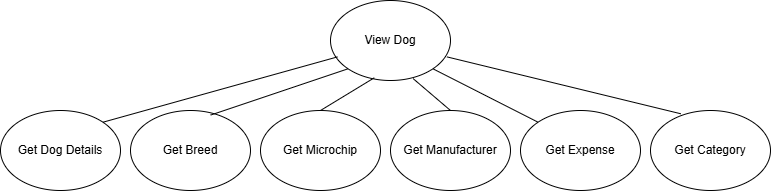
\includegraphics[width=0.8\linewidth]{task1_diagram.png}
\end{center}
\begin{itemize}
    \item \textbf{Lock Types:} Read on DOG, BREED, EXPENSE, CATEGORY, MICROCHIP, and MANUFACTURER tables.
    \item \textbf{Enabling Conditions:} User must be logged in. Dog information must be entered.
    \item \textbf{Frequency:} Often.
    \item \textbf{Schemas:} Several different schema structures needed.
    \item \textbf{Consistency:} Not critical, this is where edits are made.
    \item \textbf{Subtasks:} Mother task required, decomposition required. Order of subtasks not necessary, but they must be done (Get Dog Details, Get Breed, Get Microchip, Get Manufacturer).
\end{itemize}
\noindent\rule{8cm}{0.4pt}
\begin{itemize}
    \item Display dog profile with:
    \begin{itemize}
        \item \textbf{dogName}
        \item \textbf{breeds} (forward slash-separated in alphabetical if multiple)
        \item \textbf{sex}
        \item \textbf{altered} status
        \item \textbf{age} (displayed in years and months)
        \item \textbf{description} (if available)
        \item \textbf{manufacturer} (if applicable)
        \item \textbf{microChipID} (if applicable)
        \item \textbf{surrenderDate}
        \item \textbf{surrenderPhone} (if applicable)
        \item \textbf{byAnimalControl} status
        \item Display expenses section:
        \begin{itemize}
            \item \textbf{totalExpense} per vendor
            \item Add all \textbf{totalExpense} and display as \textbf{grandTotal}
        \end{itemize}
        \item If user.\textbf{age} is greater than 18:
        \begin{itemize}
            \item Display \textbf{Enter New Expense} link
        \end{itemize}
        \item If \textbf{user} is Director and dog.\textbf{microChipID} is not NULL and dog.\textbf{altered} is true -Display \textbf{Add Adoption} button
    \end{itemize}
\end{itemize}


\subsection{Update Dog Information}
\begin{center}
    \includegraphics[width=0.3\linewidth]{task4.png}
\end{center}
\begin{itemize}
    \item \textbf{Lock Types:} Writes on BREED, DOG, and MICROCHIP.
    \item \textbf{Enabling Conditions:} User must be logged in. Dog information must be entered. Executive Director can add adoption.
    \item \textbf{Frequency:} Often.
    \item \textbf{Schemas:} Several different schema structures needed.
    \item \textbf{Consistency:} Not critical, only one person can do this at a time.
    \item \textbf{Subtasks:} No mother task, no decomposition.
\end{itemize}
\noindent\rule{8cm}{0.4pt}
\begin{itemize}
    \item Upon:
    \begin{itemize}
        \item Click \textbf{Enter New Expense link} then jump to \textbf{Expenses} task
        \item Click \textbf{Add Application} button then jump to \textbf{Add Application} task
    \end{itemize}
    \item If a dog is adopted, disable everything
    \begin{itemize}
        \item \textbf{dogName} (Disabled)
        \item \textbf{breeds} (If unknown or mixed, editable. Otherwise, disable)
        \item \textbf{sex} (If unknown, editable. Otherwise, disable)
        \item \textbf{altered} status (If false, editable. Otherwise, disable)
        \item \textbf{age} (disabled)
        \item \textbf{description} (disabled)
        \item \textbf{manufacturer} (If null and user.age greater than 18, editable. Update microChipID dropdown.)
        \item \textbf{microChipID} (If manufacturer is not null and user.age is greater than 18, editable.)
        \item \textbf{surrenderDate} (disabled)
        \item \textbf{surrenderPhone} (disabled)
        \item \textbf{byAnimalControl} status (disabled)
    \end{itemize}
\end{itemize}

\subsection{Add Expenses}
\begin{center}
    \includegraphics[width=0.3\linewidth]{task5.png}
\end{center}
\begin{itemize}
    \item \textbf{Lock Types:} Writes on EXPENSE and reads on CATEGORY.
    \item \textbf{Enabling Conditions:} User must be logged in and at least 18.
    \item \textbf{Frequency:} Often.
    \item \textbf{Schemas:} Several different schemas required.
    \item \textbf{Consistency:} Not critical.
    \item \textbf{Subtasks:} No mother task, no decomposition.
\end{itemize}
\noindent\rule{8cm}{0.4pt}
\begin{itemize}
    \item Display form with inputs:
    \begin{itemize}
        \item \textbf{expenseDate}: calendar input
        \item \textbf{vendorName}: text box
        \item \textbf{amount}: double
        \item \textbf{expenseCategory}: dropdown
    \end{itemize}
    \item Submission conditions:
    \begin{itemize}
        \item If dog has not been adopted and dog is surrendered:
        \begin{itemize}
            \item Allow submit
        \end{itemize}
        \item If (\textbf{expenseCategory} exists and \textbf{currentDate} is true) OR user.\textbf{age} is less than 18:
        \begin{itemize}
            \item Do not allow submit
        \end{itemize}
    \end{itemize}
\end{itemize}

\subsection{Adoption Review}
\begin{center}
    \includegraphics[width=0.2\linewidth]{task6.png}
\end{center}
\begin{itemize}
    \item \textbf{Lock Types:} Reads on ADOPTER and APPLICATION. Writes on APPLICATION.
    \item \textbf{Enabling Conditions:} User must be logged in and must be executive director.
    \item \textbf{Frequency:} Number of adoption applications submitted.
    \item \textbf{Schemas:} Several different schemas required.
    \item \textbf{Consistency:} Not critical.
    \item \textbf{Subtasks:} Mother task required, decomposition required. Order of subtasks not necessary, but they must be done (Find Applications).
\end{itemize}
\noindent\rule{8cm}{0.4pt}
\begin{itemize}
    \item Display pending applications and applicant contact information.
    \item Display table containing:
    \begin{itemize}
        \item Applications in \textbf{Pending} state.
        \item Applicant contact details:
        \begin{itemize}
            \item \textbf{firstName}
            \item \textbf{lastName}
            \item \textbf{Address}:
            \begin{itemize}
                \item \textbf{street}
                \item \textbf{city}
                \item \textbf{state}
                \item \textbf{zipCode}
            \end{itemize}
            \item \textbf{phoneNumber}
            \item \textbf{emailAddress}
        \end{itemize}
        \item Buttons for:
        \begin{itemize}
            \item \textbf{Approve}
            \item \textbf{Reject}
        \end{itemize}
    \end{itemize}
\end{itemize}


\subsection{Add Application}
\begin{center}
    \includegraphics[width=0.3\linewidth]{task7.png}
\end{center}
\begin{itemize}
    \item \textbf{Lock Types:} Writes on APPLICATION and ADOPTER.
    \item \textbf{Enabling Conditions:} User must be logged in.
    \item \textbf{Frequency:} Amount of dogs adopted.
    \item \textbf{Schemas:} Several different schemas required.
    \item \textbf{Consistency:} Critical, need to be sure we don't do two applications a day.
    \item \textbf{Subtasks:} No mother task, no decomposition.
\end{itemize}
\noindent\rule{8cm}{0.4pt}
\begin{itemize}
    \item Display form with inputs:
    \begin{itemize}
        \item \textbf{firstName}: text box
        \item \textbf{lastName}: text box
        \item \textbf{street}: text box
        \item \textbf{city}: text box
        \item \textbf{state}: text box
        \item \textbf{zipCode}: number input (numbers only)
        \item \textbf{phoneNumber}: number input (numbers only)
        \item \textbf{emailAddress}: text box
        \item \textbf{householdSize}: number input (numbers only)
    \end{itemize}
    \item \textbf{applicationStatus} will be set to "Pending" upon submission.
    \item Submission conditions:
    \begin{itemize}
        \item If \textbf{emailAddress} and \textbf{dateOfApplication} exist:
        \begin{itemize}
            \item Display error message indicating only one application per day is allowed.
        \end{itemize}
    \end{itemize}
\end{itemize}


\subsection{Search Applications}
\begin{center}
    \includegraphics[width=0.6\linewidth]{task8.png}
\end{center}
\begin{itemize}
    \item \textbf{Lock Types:} Read on APPLICATION, EXPENSE, and DOG.
    \item \textbf{Enabling Conditions:} User must be logged in and must be executive director.
    \item \textbf{Frequency:} Amount of dogs adopted approved.
    \item \textbf{Schemas:} Several different schema structures needed.
    \item \textbf{Consistency:} Critical, needs to reflect all applications for the dog.
    \item \textbf{Subtasks:} Mother task required, decomposition required. Order of subtasks not necessary, but they must be done (Get Dog Details, Calculate Expenses, Find Applications).
\end{itemize}
\noindent\rule{8cm}{0.4pt}
\begin{itemize}
    \item Display search input box:
    \begin{itemize}
        \item Look up via applicant's 	\textbf{lastName} (case insensitive)
    \end{itemize}
    \item Display list of applicants with:
    \begin{itemize}
        \item 	\textbf{firstName} + 	\textbf{lastName} (clickable link)
        \item Address: 	\textbf{street}, 	\textbf{city}, 	\textbf{state}, 	\textbf{zipCode}
        \item 	\textbf{phoneNumber}
        \item 	\textbf{emailAddress}
        \item 	\textbf{householdSize}
    \end{itemize}
    \item Upon selecting an applicant (via 	\textbf{firstName} + 	\textbf{lastName} link):
    \begin{itemize}
        \item Display most recent application
        \item Calculate and display 	\textbf{adoptionFee}:
        \begin{itemize}
            \item If dog's 	\textbf{breeds} contains "Terrier" and dog's 	\textbf{name} is "Sideways", set 	\textbf{adoptionFee} to 0
        \end{itemize}
    \end{itemize}
\end{itemize}


\subsection{Set Adoption Date}
\begin{center}
    \includegraphics[width=0.3\linewidth]{task9.png}
\end{center}
\begin{itemize}
    \item \textbf{Lock Types:} Writes on APPLICATION.
    \item \textbf{Enabling Conditions:} User must be logged in and must be executive director.
    \item \textbf{Frequency:} Amount of dogs adopted approved.
    \item \textbf{Schemas:} Several different schema structures needed.
    \item \textbf{Consistency:} Not critical.
    \item \textbf{Subtasks:} No mother task, no decomposition.
\end{itemize}
\noindent\rule{8cm}{0.4pt}
\begin{itemize}
\item Upon entering 	\textbf{adoptionDate}:
\begin{itemize}
    \item Display confirmation screen with:
    \begin{itemize}
        \item Dog name
        \item Adopter contact info
        \item Adoption fee
        \item Adoption date
    \end{itemize}
    \item Display 	\textbf{Submit} button:
    \begin{itemize}
        \item Disabled if 	\textbf{microchipId} is null and 	\textbf{altered} is false
    \end{itemize}
\end{itemize}        
\end{itemize}        


\subsection{View Dog Dashboard}
\begin{center}
    \includegraphics[width=0.5\linewidth]{task10.png}
\end{center}
\begin{itemize}
    \item \textbf{Lock Types:} Read on DOG.
    \item \textbf{Enabling Conditions:} User must be logged in.
    \item \textbf{Frequency:} Number of dogs and applications being added per day.
    \item \textbf{Schemas:} Several different schema structures needed.
    \item \textbf{Consistency:} Critical, need to know if dog has been adopted.
    \item \textbf{Subtasks:} Mother task required, decomposition required. Order of subtasks not necessary, but they must be done (List Dogs, Calculate Space).
\end{itemize}
\noindent\rule{8cm}{0.4pt}
\begin{itemize}
    \item Calculable available space:
    \begin{itemize}
        \item \textbf{availableSpace} = \textbf{maxCapacity} - \textbf{currentNumberOfDogs}
    \end{itemize}
    \item Display the following:
    \begin{itemize}
        \item \textbf{Add Adoption Application} button
        \item If \textbf{maxCapacity} is greater than \textbf{currentNumberOfDogs}
        \begin{itemize}
            \item Display \textbf{Add Dog} button 
        \end{itemize}
        \item \textbf{Filter} dropdown
    \end{itemize}
    \item If user is a director:
    \begin{itemize}
        \item Display the following:
        \begin{itemize}
            \item \textbf{Adoption Application Review} button
            \item \textbf{Animal Control Report} button
            \item \textbf{Monthly Adoption Report} button
            \item \textbf{Expense Analysis} button
            \item \textbf{Volunteer Lookup} button
            \item \textbf{Volunteer Birthdays} button
        \end{itemize}
    \end{itemize}
    \item Display Available Space: \{\textbf{availableSpace}\}
    \item Display all dogs currently in shelter in a table:
    \begin{itemize}
        \item Columns: \textit{dogName} (clickable link), \textit{breeds}, \textit{sex}, \textit{altered}, \textit{age}, and \textit{adoptability}
        \item Order dogs oldest to newest by \textit{surrenderDate}
    \end{itemize}
    \item If user selects a value from the \textbf{Filter} dropdown:
    \begin{itemize}
        \item If value is adoptable:
        \begin{itemize}
            \item Display in table dogs that are only adoptable
        \end{itemize}
        \item Else if value is not adoptable:
        \begin{itemize}
            \item Display in table dogs that are not adoptable
        \end{itemize}
        \item Else if value is All (default):
        \begin{itemize}
            \item Display all dogs in table
        \end{itemize}
    \end{itemize}
    \item Upon:
    \begin{itemize}
        \item Click \textbf{dogName} link - Jump to the \textbf{Dog Detail} task
        \item Click \textbf{Adoption Application Review} button - Jump to the \textbf{Adoption Application Review} task
        \item Click \textbf{Animal Control Report} button - Jump to the \textbf{Animal Control Report} task
        \item Click \textbf{Monthly Adoption Report} button - Jump to the \textbf{Monthly Adoption Report} task
        \item Click \textbf{Expense Analysis} button - Jump to the \textbf{Expense Analysis} task
        \item Click \textbf{Volunteer Lookup} button - Jump to the \textbf{Volunteer Lookup} task
        \item Click \textbf{Volunteer Birthdays} button - Jump to the \textbf{Volunteer Birthdays} task
        \item Click \textbf{Add Adoption Application} button - Jump to the \textbf{Add Adoption Application} task
        \item Click \textbf{Add Dog} button - Jump to the \textbf{Add Dog} task
    \end{itemize}
\end{itemize}

\subsection{View Animal Control Report}
\begin{center}
    \includegraphics[width=0.5\linewidth]{task11.png}
\end{center}
\begin{itemize}
    \item \textbf{Lock Types:} Read on DOG, BREEDS, MICROCHIP, CATEGORY, and EXPENSE.
    \item \textbf{Enabling Conditions:} User must be logged in and be executive director.
    \item \textbf{Frequency:} At least monthly.
    \item \textbf{Schemas:} Several different schema structures needed.
    \item \textbf{Consistency:} Critical to the day.
    \item \textbf{Subtasks:} Mother task required, decomposition required. Order of subtasks not necessary, but they must be done (Filter Dogs, Calculate Expenses).
\end{itemize}
\noindent\rule{8cm}{0.4pt}
\begin{itemize}
\item Display table with:
\begin{itemize}
    \item Rows: One for each month (current month plus previous 6 months):
    \item Columns:
    \begin{itemize}
        \item Month (start/end dates)
        \item Count of dogs surrendered by animal control (clickable)
        \item Count of dogs adopted after 60+ days in rescue (clickable)
        \item Total expenses for adopted dogs
        \item If dog.\textbf{byAnimalControl} is true:
        \begin{itemize}
            \item exclude from expense
        \end{itemize}
        \item Current month row shows data up to current date
        \item Each count/total is clickable and displays corresponding drill-down report
    \end{itemize}
    \item Upon clicking a cell, display corresponding drill-down report:
\end{itemize}        
    \begin{itemize}
        \item \textbf{Animal Control Surrenders Drill Down}
        \begin{itemize}
            \item Display table with columns:
            \begin{itemize}
                \item \textbf{dogID}
                \item \textbf{breeds} (forward slash-separated in alphabetical if multiple)
                \item \textbf{sex}
                \item \textbf{altered}
                \item \textbf{microChipID}
                \item \textbf{surrenderDate}
            \end{itemize}
            \item Sort by \textbf{dogID} ascending
        \end{itemize}
    \end{itemize}
    \begin{itemize}
        \item \textbf{Dogs Adopted (60+ days) Drill-down}
        \begin{itemize}
            \item Display table with columns:
            \begin{itemize}
                \item \textbf{dogID}
                \item \textbf{breeds} (forward slash-separated in alphabetical if multiple)
                \item \textbf{sex}
                \item \textbf{microChipID}
                \item \textbf{surrenderDate}
                \item \textbf{daysInRescue} (count includes both surrender and adoption dates)
            \end{itemize}
            \item Sort \textbf{daysInRescue} descending then \textbf{dogID} descending
        \end{itemize}
    \end{itemize}
    \begin{itemize}
        \item \textbf{Adopted Dogs Expenses Drill-down}
        \begin{itemize}
            \item Display table with columns:
            \begin{itemize}
                \item \textbf{dogID}
                \item \textbf{breeds} (forward slash-separated in alphabetical if multiple)
                \item \textbf{sex}
                \item \textbf{microChipID}
                \item \textbf{surrenderDate}
                \item \textbf{byAnimalControl} indicator
                \item \textbf{totalExpenses} (exclude from expense if dog.byAnimalControl is true)
            \end{itemize}
            \item Sort by \textbf{dogID} ascending
        \end{itemize}
    \end{itemize}
\end{itemize} 

\subsection{View Adoption Report}
\begin{center}
    \includegraphics[width=0.7\linewidth]{task12.png}
\end{center}
\begin{itemize}
    \item \textbf{Lock Types:} Read on DOG, BREEDS, and EXPENSE.
    \item \textbf{Enabling Conditions:} User must be logged in and be executive director.
    \item \textbf{Frequency:} At least yearly.
    \item \textbf{Schemas:} Several different schema structures needed.
    \item \textbf{Consistency:} Not critical.
    \item \textbf{Subtasks:} Mother task required, decomposition required. Order of subtasks not necessary, but they must be done (Calculate Number of Dogs, Calculate Adoption Fees, Calculate Total Expenses, Calculate Net Profit).
\end{itemize}
\noindent\rule{8cm}{0.4pt}
\begin{itemize}
\item Display table for previous 12 months (excluding current month):
\begin{itemize}
    \item Columns:
    \begin{itemize}
        \item Month/Year
        \item Number of dogs surrendered
        \item Number of dogs adopted
        \item Total expenses (exclude from expense if dog.byAnimalControl is true)
        \item Total adoption fees (Calculate Per Dog)
        \begin{itemize}
            \item If \textbf{dog.byAnimalControl} is true: (\textbf{adoptionFee} = \textbf{totalExpenses} / 0.10)
            \item Else: (\textbf{adoptionFee} = \textbf{totalExpenses} / 1.25)
        \end{itemize}
        \item Net Profit:
        \begin{itemize}
            \item \textbf{totalAdoptionFees} - \textbf{totalExpenses}
        \end{itemize}
        \item Group Rows by Breed:
        \begin{itemize}
            \item Show only breeds adopted/surrendered in 12-month period
            \item For multiple breeds, combine names alphabetically with delimiter
        \end{itemize}
        \item Sort by:
        \begin{itemize}
            \item Month ascending (earliest to latest)
            \item Breed name alphabetically
        \end{itemize}
    \end{itemize}
\end{itemize}        
\end{itemize}    


\subsection{View Expense Analysis Report}
\begin{center}
    \includegraphics[width=0.5\linewidth]{task13.png}
\end{center}
\begin{itemize}
    \item \textbf{Lock Types:} Reads on DOG and EXPENSE.
    \item \textbf{Enabling Conditions:} User must be logged in and be executive director.
    \item \textbf{Frequency:} Often.
    \item \textbf{Schemas:} Several different schema structures needed.
    \item \textbf{Consistency:} Not critical.
    \item \textbf{Subtasks:} Mother task required, decomposition required. Order of subtasks not necessary, but they must be done (Set Vendor, Calculate Expenses).
\end{itemize}
\noindent\rule{8cm}{0.4pt}
\begin{itemize}
\item Display table with::
\begin{itemize}
    \item \textbf{vendorName}:
    \begin{itemize}
        \item If dog.\textbf{byAnimalControl} is true
        \begin{itemize}
            \item Exclude from expenses
        \end{itemize}
        \item Sort by \textbf{totalExpenses} descending:
    \end{itemize}
\end{itemize}        
\end{itemize}   

\subsection{View Volunteer Lookup Report}
\begin{center}
    \includegraphics[width=0.2\linewidth]{task14.png}
\end{center}
\begin{itemize}
    \item \textbf{Lock Types:} Read on VOLUNTEER and PERSON.
    \item \textbf{Enabling Conditions:} User must be logged in and be executive director.
    \item \textbf{Frequency:} Often.
    \item \textbf{Schemas:} Single.
    \item \textbf{Consistency:} Not critical.
    \item \textbf{Subtasks:} Mother task required, decomposition required. Order of subtasks not necessary, but they must be done (Set Person).
\end{itemize}
\noindent\rule{8cm}{0.4pt}
\begin{itemize}
\item Search by first or last name containing (case insensitive)
\begin{itemize}
    \item Display:
    \begin{itemize}
        \item First name
        \item Last name
        \item Email address
        \item Phone number
    \end{itemize}
    \item Sort by last name ascending, first name ascending
\end{itemize}        
\end{itemize}    


\subsection{View Volunteer Birthdays Report}
\begin{center}
    \includegraphics[width=0.3\linewidth]{task15.png}
\end{center}
\begin{itemize}
    \item \textbf{Lock Types:} Reads on VOLUNTEER and PERSON.
    \item \textbf{Enabling Conditions:} User must be logged in and be executive director.
    \item \textbf{Frequency:} Daily.
    \item \textbf{Schemas:} Single.
    \item \textbf{Consistency:} Not critical.
    \item \textbf{Subtasks:} No mother task, no decomposition.
\end{itemize}
\noindent\rule{8cm}{0.4pt}
\begin{itemize}
    \item Display month/year selection:
    \begin{itemize}
        \item Dropdown with all months
        \item Year options limited to current and previous year
        \item Default to current month/year
    \end{itemize}
    \item For selected month:
    \begin{itemize}
        \item If no birthdays: Display message "No volunteer birthdays this month!"
        \item If birthdays exist, display table with:
        \begin{itemize}
            \item \textbf{firstName}
            \item \textbf{lastName}
            \item \textbf{emailAddress}
            \item \textbf{milestoneBirthday} (Yes/No for ages divisible by 10)
        \end{itemize}
    \end{itemize}
    \item Sort by \textbf{lastName} ascending, then \textbf{firstName} ascending
\end{itemize}

\end{document}
